%------------------------------------------------
\section{Éxistants}
%------------------------------------------------

%-----------------------------------------------------------------
\subsection{Suivi de bord}
%-----------------------------------------------------------------

\begin{frame}
\frametitle{Suivi de bord}


\begin{columns}[t]
  \begin{column}{0.6\linewidth}
    \begin{block}{Cas particulier d'$\alpha-shape$ - $\alpha = -\sqrt{2}$}
      Ensemble de sommets consécutifs récupérant le bord 4-connexe du disque.\\
      Méthode incrémentale :
      \begin{enumerate}
        \item<2-> Trouver un point de départ sur le bord.
        \item<3> Chercher le point adjacent suivant.
      \end{enumerate}
    \end{block}
    \only<2>
    {
      \begin{block}{Point de départ}
        Recherche du point à l'intérieur d'ordonnée minimale et d'abscisse maximale.\\
        \begin{itemize}
          \item Départ du point avec les coordonnées entières du centre.
          \item Descente d'une longueur égale au rayon.
          \item Translation vers la droite la plus grande possible.
        \end{itemize}
      \end{block} 
    }
    \only<3>
    {
      \begin{block}{Point suivant}
        En partant d'un voisin à l'extérieur, le point suivant est le premier voisin à l'intérieur. 
        \begin{itemize}
          \item Sens de rotation.
          \item Connexité souhaitée.
        \end{itemize}
      \end{block} 
    }
  \end{column}
  \begin{column}{0.4\linewidth}
    \only<1>
    {
      \begin{figure}[h!]
        \centering
        \includegraphics[width=0.8\linewidth]{fig/2-mot/as/mot-as-1.pdf}
      \end{figure}    
    }
    \only<2>
    {
      \begin{figure}[h!]
        \centering
        \includegraphics[width=0.8\linewidth]{fig/3-exi/suivi/exi-depart.pdf}
      \end{figure}    
    }
    \only<3>
    {  
      \begin{figure}[h!]
        \centering
        \includegraphics[width=0.9\linewidth]{fig/3-exi/suivi/exi-suivi-2.pdf}
      \end{figure}  
    }
  \end{column}
\end{columns}





\end{frame}

%-----------------------------------------------------------------
\subsection{Enveloppe Convexe}
%-----------------------------------------------------------------

\begin{frame}
\frametitle{Enveloppe Convexe}
\begin{block}{Algorithme de Graham}
  \only<1>
  {
  Soit n le nombre d'éléments de $\mathcal{D}$.
  Principe :
  \begin{enumerate}
    \item Trier les n points. Complexité en $O(n \log n)$
    \item Marche de Graham : Etude de l'orientation du sommet suivant par rapport au deux précédents. Complexité en $O(n)$
  \end{enumerate}

  \begin{itemize}
    \item L'ensemble de point sur le bord 4-connexe : S est déjà triés.\\
    On n'effectue que la marche de Graham.
    \item Il y a \#S = 4R sommets sur le bord 4-connexes.
    \item Complexité en $O(R)$.
  \end{itemize}
  
 }
 \only<2> 
  {
  \begin{itemize}
    \item Complexité en $O(R)$.
  \end{itemize}
 }  
\end{block}

\only<1>
{
  %----- Begin biblio -----
  \scriptsize
  \begin{thebibliography}{alpha}
    \bibitem{Graham1972}
    [Graham1972] Graham, Ronald L.
    \newblock Convex hull algorithm
    \newblock {\em Inf. Process. Lett.}, 1972. 
  \end{thebibliography}
  %----- End biblio   -----
}
\only<2>
{
  \begin{block}{Har-Peled}  
    Méthode géométrique qui construit successivement les arêtes du polygone à l’aide des convergents.
    \begin{itemize}
      \item Incrémental.
      \item Output Sensitive.\\
      Dépend du nombre de sommets de l’enveloppe convexe.
    \end{itemize}  

    \begin{itemize}
      \item Complexité de la recherche du prochain sommet en $O(\log R)$
      \item Nombre de sommets en $O(R^{2/3})$. 
    \end{itemize}
    Complexité en $O(R^{2/3} \log R)$.
  \end{block}

  %----- Begin biblio -----
  \scriptsize
  \begin{thebibliography}{alpha}
    \bibitem{HarPeled98}
    [HarPeled98] Har-Peled
    \newblock An Output Sensitive Algorithm for Discrete Convex Hulls
    \newblock {\em ICGTA: Computational Geometry: Theory and Applications}, 1998.
    \end{thebibliography}
  %----- End biblio   -----
}
\end{frame}



\begin{frame}
\frametitle{Har Peled - Enveloppe Convexe de Disques}

\begin{block}{Principes de l'algorithme}
  \begin{enumerate}
    \item Trouver un point de départ sur le bord.\\
    \only{Même méthode que précédement.}
    \item Chercher le prochain sommet de l'enveloppe convexe à l'aide des convergents.\\
  \end{enumerate}
\end{block}

\begin{block}{Calcul des convergents}
  Soient :\\
  $p_{-2} = (1,0)$ et $p_{-1} = (0,1)$.
  Calcul réccursif : \\
  \alert{$$p_{k} = p_{k-2} + q_k p_{k-1}$$}
  $q_k$ est le plus grand entier tel que $p_{k}$ et $p_{k-1}$ sont de part et d'autre du cercle.
\end{block}
\end{frame}

\begin{frame}
\frametitle{Har Peled - Enveloppe Convexe de Disques}

\begin{columns}[t]
  \begin{column}{0.7\linewidth}
    \begin{block}{Convergents}
      
      \begin{columns}[t]
        \begin{column}{0.6\linewidth}
          \alert{$$p_{k} = p_{k-2} + q_k p_{k-1}$$}\\
          $p_{k}$ et $p_{k-1}$ sont de part et d'autre du cercle.
          \begin{itemize}
            \item k impairs : $p_k \in \mathcal{D}$.
            \item k pairs : $p_k \not\in \mathcal{D}$.
          \end{itemize}
        \end{column}
        \begin{column}{0.4\linewidth}
        $p_{-2} = (1,0)$\\
        $p_{-1} = (0,1)$\\
        \only<2-4>{$p_{0} = ?$\\}
        \only<5->{$p_{0} = (1,2)$\\}
        \only<6-8>{$p_{1} = ?$\\}
        \only<9->{$p_{1} = (2,5)$\\}
        \only<10>{$p_{2} = ?$\\}
        \end{column}
      \end{columns}     
    \end{block}  
     \begin{block}{Choix du prochain sommet}   
      \begin{enumerate}
        \item Le convergent se situe exactement sur le bord du disque.
        \item Le convergent a le plus grand degré impair lorsque que le lancer de rayon n’intersecte plus le disque.
      \end{enumerate}
    \end{block}     
  \end{column}
  
  \begin{column}{0.3\linewidth}
    \only<1>
    {
      \begin{figure}[H]
        \centering
        \includegraphics[width=.9\linewidth]{fig/3-exi/har/exi-har-0.pdf}
      \end{figure}
    }
    \only<2>
    {
      \begin{figure}[H]
        \centering
        \includegraphics[width=.9\linewidth]{fig/3-exi/har/exi-har-1.pdf}
      \end{figure}
    }
    \only<3>
    {
      \begin{figure}[H]
        \centering
        \includegraphics[width=.9\linewidth]{fig/3-exi/har/exi-har-2.pdf}
      \end{figure}
    }
    \only<4>
    {
      \begin{figure}[H]
        \centering
        \includegraphics[width=.9\linewidth]{fig/3-exi/har/exi-har-3.pdf}
      \end{figure}
    }
    \only<5>
    {
      \begin{figure}[H]
        \centering
        \includegraphics[width=.9\linewidth]{fig/3-exi/har/exi-har-4.pdf}
      \end{figure}
    }
    \only<6>
    {
      \begin{figure}[H]
        \centering
        \includegraphics[width=.9\linewidth]{fig/3-exi/har/exi-har-5.pdf}
      \end{figure}
    }
    \only<7>
    {
      \begin{figure}[H]
        \centering
        \includegraphics[width=.9\linewidth]{fig/3-exi/har/exi-har-6.pdf}
      \end{figure}
    }
    \only<8>
    {
      \begin{figure}[H]
        \centering
        \includegraphics[width=.9\linewidth]{fig/3-exi/har/exi-har-7.pdf}
      \end{figure}
    }
    \only<9>
    {
      \begin{figure}[H]
        \centering
        \includegraphics[width=.9\linewidth]{fig/3-exi/har/exi-har-8.pdf}
      \end{figure}
    }
    \only<10>
    {
      \begin{figure}[H]
        \centering
        \includegraphics[width=.9\linewidth]{fig/3-exi/har/exi-har-9.pdf}
      \end{figure}
    }
    \only<11>
    {
      \begin{figure}[H]
        \centering
        \includegraphics[width=.9\linewidth]{fig/3-exi/har/exi-har-10.pdf}
      \end{figure}
    }  
  \end{column}
\end{columns}
\end{frame}

\begin{frame}
\frametitle{Résultats}

\begin{block}{}
  \textbf{Protocole} : 100 disques de rayon $R = 2^k$, $k = \{5,...,28\}$ et de centre rationnel aléatoire appartenant à $[0,1]\times[0,1]$.
\end{block}


\begin{columns}[t]
%---- col 1 
  \begin{column}{0.2\linewidth}
    \vspace{-0.8cm}
    \begin{tiny}
      \begin{table}[H]
        \begin{tabular}{|p{0.018cm}|p{0.8cm}|p{0.25cm}|}
          \hline
          k  & $\#$      & $/ R^{2/3}$ \\    
          \hline
          5  & 35,36     & 3,51\\
          6  & 55,78     & 3,49\\
          7  & 87,78     & 3,46\\
          8  & 139,71    & 3,47\\
          9  & 222,07    & 3,47\\
          10 & 351,72    & 3,46\\
          11 & 558,18    & 3,46\\
          12 & 883,86    & 3,45\\
          13 & 1,40E+003 & 3,45\\
          14 & 2,23E+003 & 3,45\\
          15 & 3,54E+003 & 3,45\\
          16 & 5,62E+003 & 3,46\\
          17 & 8,91E+003 & 3,45\\
          18 & 1,41E+004 & 3,45\\
          19 & 2,25E+004 & 3,45\\
          20 & 3,56E+004 & 3,45\\
          21 & 5,66E+004 & 3,45\\
          22 & 8,98E+004 & 3,45\\
          23 & 1,43E+005 & 3,45\\
          24 & 2,26E+005 & 3,45\\
          25 & 3,59E+005 & 3,45\\
          26 & 5,70E+005 & 3,45\\
          27 & 8,98E+005 & 3,42\\
          28 & 1,35E+06  & 3,24\\
          \hline
        \end{tabular} 
        \label{tab:ch} 
      \end{table}
    \end{tiny}
  \end{column}
%---- col 2 
  \begin{column}{0.8\linewidth}
    \vspace{-0.6cm}
    \only<1>
    {
      \begin{figure}[H]
        \centering
        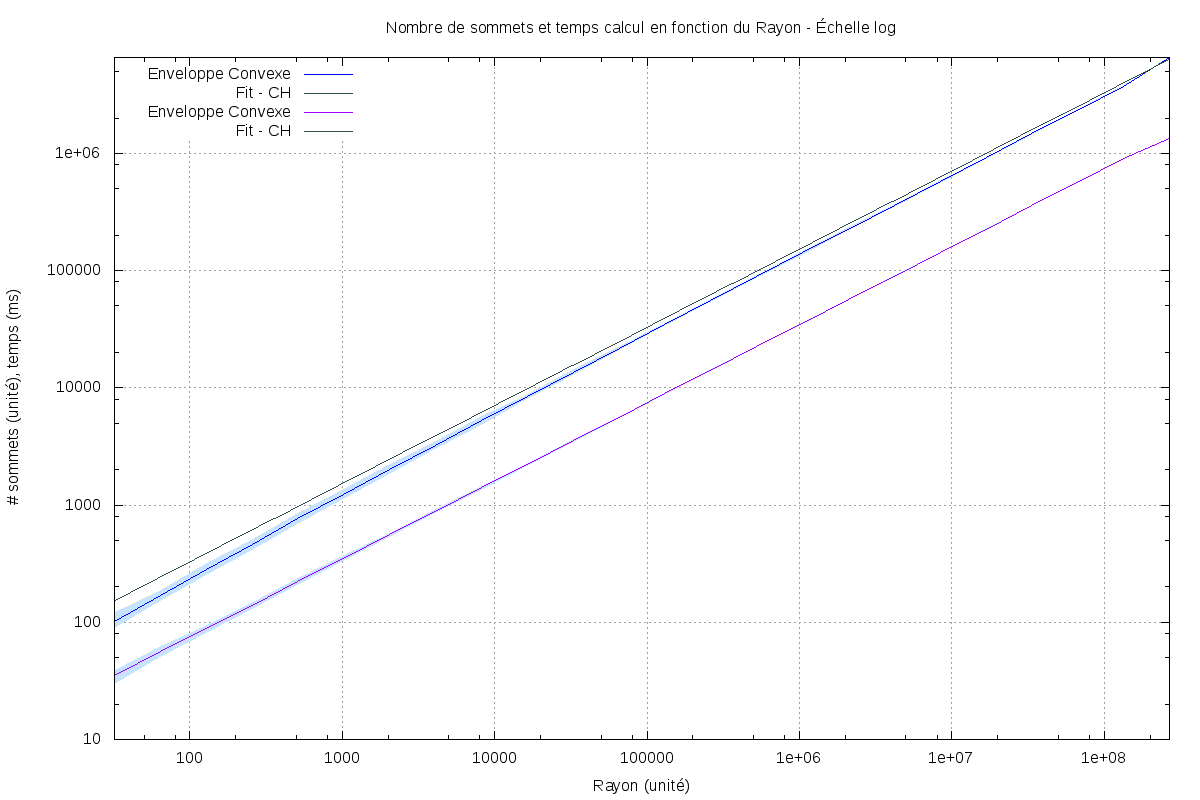
\includegraphics[width=0.7\linewidth]{fig/3-exi/har/exi-ch-sommet.png}       
      \end{figure}
      \vspace{-0.3cm}
      \begin{exampleblock}{}
       \textbf{Nombre de sommet de l'enveloppe convexe}\\
        La division du nombre de sommets par $R^{2/3}$ se stabilise.\\
        Le nombre de sommet \textbf{converge asymptotiquement} en $O(R^{2/3})$. \\
        Nombre de sommets $ \approx 3.45 * R^{2/3}$.\\
        Les résultats sont conformes à la publication. \\

     \end{exampleblock}
    }
    
    \only<2>
    {
      \begin{figure}[H]
        \centering
        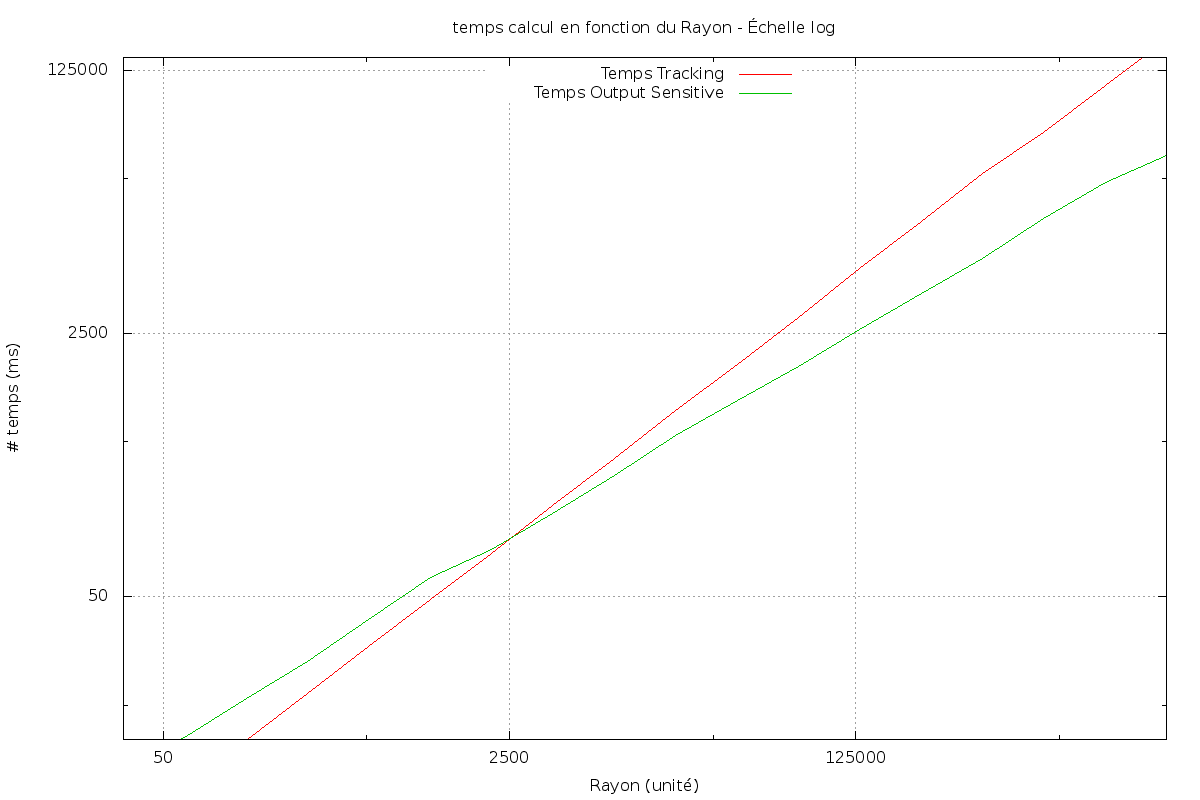
\includegraphics[width=0.7\linewidth]{fig/3-exi/har/exi-ch-temps.png}
      \end{figure}
      \vspace{-0.3cm}
      \begin{exampleblock}{}
        \textbf{Compléxité en temps}\\
        Rapidement  ($R \approx 900$) la méthode de Har-Peled (\textit{sous-linéaire}) devient plus intéressante que la marche de Graham (\textit{linéaire}).\\
        Les résultats sont conformes à la publication.
      \end{exampleblock}
    }
       
  \end{column}  
\end{columns}
\end{frame}
